\chapter{The Most Important Chapter}
\section{Here be random text about \textsc{srt/lrt}}
This is a test. Let's see how this goes! Btw, $e^{i\pi} = -1$ and $(\partial_\mu \partial^\mu - m^2) \psi = 0$.
Also $\partial_z I = \partial_z \Delta = 0$.
%Also, we know well that $I(\varphi) = I_0 \sin \varphi$.  And also $\mathbf{R}\mathbb{R} \otimes \mathbf{C}\mathbb{C} \oplus \mathbf{N}\mathbb{N}_+$.\footnote{This is simply just a simple test, with an equation $\sin a = \cos(2b-1)/\cos(2b+1)$. And here is a chemical element \ce{CrO23} and physical unit \SI{12e3}{m}. }
%Also we can point out $I = \{ 1 \pm [\sin(a)\tan(b)]^2\} $.
Here is another equation:
\begin{equation}
  Δ(z) = \int_0^{ω_c} \mathrm{d}ε\;\mathrm{Re}\; f_s(ε) \tanh\!\left(\frac{π}{2e^γ} \frac{ε/Δ_0}{T/T_c}\right)
\end{equation}
\begin{equation}
  \Delta(z) = \int_0^{\omega_c} \mathrm{d}\epsilon\,\mathrm{Re}\, f_s(\epsilon) \tanh\!\left(\frac{\pi}{2e^\gamma} \frac{\epsilon/\Delta_0}{T/T_c}\right)
\end{equation}
Here is some normal text. \textit{And here is some emphasized text 1234567890}. Normal 123456789. 
Say something about the \textsc{bcs} theory and \textsc{bcs-bec} transition \emph{and \textsc{srt/lrt} in italics}.
This is another test: $1 < 2 > 0 \leq 1 \geq 2$, and here is an url: \url{http://www.google.com/interesting_something/else/and/even/more/stuff}
%\verb+for i=[0:0.1:1.0] do f(i,j) = 1/g(j,i)+
\begin{equation}
  \textit{e}e\mathrm{e}\textsf{e}%\texttt{e}\;
  \textit{I}I\mathrm{I}\textsf{I}%\texttt{I}\;
  \textit{m}m\mathrm{m}\textsf{m}%\texttt{m}
\end{equation}
\textsf{And here is some sans-serif text with math $e^{i\varphi}=\cos\varphi+i\sin\varphi$ and so on.} And here is some normal text again.
Here is a chemical equation \ce{CrO23} and unit \SI{23e23}{m/s} but $J_0 = \SI{23e23}{m/s}$ also.

%\subsection{Miscellaneous symbols}
%\begin{equation}
%\mathbf{ABCDEFGHIJKLMOPQRSTUVWXYZ}
%\end{equation} 
%\begin{equation}
%\mathbf{abcdefghijklmnopqrstuvwxyz}
%\end{equation} 
%\begin{equation}
%ABCDEFGHIJKLMOPQRSTUVWXYZ
%\end{equation} 
%\begin{equation}
%abcdefghijklmopqrstuvwxyz
%\end{equation} 
%\begin{equation}
%\alpha\beta\gamma\delta\varepsilon\theta\vartheta\phi\varphi\psi\eta\kappa\lambda
%\end{equation} 
%\begin{equation}
%\Gamma\Delta\Theta\Phi\Psi\Lambda
%\end{equation} 
%\begin{equation}
%\mathbf{\alpha\beta\gamma\delta\epsilon\varepsilon\theta\vartheta\phi\varphi\psi\eta\kappa\lambda\sigma}
%\end{equation} \begin{equation}
%\mathbf{\Gamma\Delta\Theta\Phi\Psi\Lambda}
%\end{equation}

%\section{Miscellaneous text (Classico)}
%This piece of text is typeset using the \textsc{newpxtext} font, with an inline equation $e^{i\varphi} = \cos\varphi + i\sin\varphi$ that uses the \textsc{euler} font. \emph{This text is italic.}\\[1ex]
%\textsf{This piece of text is typeset using the CLASSICO (OPTIMA) font, with an inline equation $e^{i\varphi} = \cos\varphi + i\sin\varphi$ that uses the \textsc{euler} font. \textit{This text is italic.}}\footnote{This is another footnote test.}
%
%\subsection{Introduction to the Usadel difficult diffusion equation}
%\subsection{Test}
%\lettrine[lraise=0.15,nindent=0.1em]{\textin{T}}{he Usadel equation} is quite interesting.
%Donec malesuada magna sem.
%Fusce vitae lectus id magna convallis euismod.
%Quisque viverra sollicitudin turpis, vel ultricies mauris dictum quis.
%Praesent justo nunc, luctus in lectus in, placerat tempus orci.
%Donec placerat neque ac tortor dignissim pellentesque.
%Aenean tellus erat, eleifend id interdum a, volutpat et massa.
%Quisque tristique accumsan efficitur.
%
%\subsection{Test}
%\lettrine[lraise=0.15,nindent=0.1em]{H}{owever, } we still have something to discuss..
%Donec malesuada magna sem.
%Fusce vitae lectus id magna convallis euismod.
%Quisque viverra sollicitudin turpis, vel ultricies mauris dictum quis.
%Praesent justo nunc, luctus in lectus in, placerat tempus orci.
%Donec placerat neque ac tortor dignissim pellentesque.
%Aenean tellus erat, eleifend id interdum a, volutpat et massa.
%Quisque tristique accumsan efficitur.
%
%\subsection{Test}
%\lettrine[lraise=0.15,nindent=0.1em]{\textin{I}}{nteresting materials} have special uses.
%Donec malesuada magna sem.
%Fusce vitae lectus id magna convallis euismod.
%Quisque viverra sollicitudin turpis, vel ultricies mauris dictum quis.
%Praesent justo nunc, luctus in lectus in, placerat tempus orci.
%Donec placerat neque ac tortor dignissim pellentesque.
%Aenean tellus erat, eleifend id interdum a, volutpat et massa.
%Quisque tristique accumsan efficitur.
%
%\subsection{Test}
%\lettrine[lraise=0.15,nindent=0.1em]{\textin{W}}{hat other people consider normal.}
%Donec malesuada magna sem.
%Fusce vitae lectus id magna convallis euismod.
%Quisque viverra sollicitudin turpis, vel ultricies mauris dictum quis.
%Praesent justo nunc, luctus in lectus in, placerat tempus orci.
%Donec placerat neque ac tortor dignissim pellentesque.
%Aenean tellus erat, eleifend id interdum a, volutpat et massa.
%Quisque tristique accumsan efficitur.

\section{Lorem ipsum}
Lorem ipsum dolor sit amet, consectetuer adipiscing elit.
Donec malesuada magna sem.
Fusce vitae lectus id magna convallis euismod.
Quisque viverra sollicitudin turpis, vel ultricies mauris dictum quis.
Praesent justo nunc, luctus in lectus in, placerat tempus orci.
\begin{equation}
  f(x) = \sin(x) + 1/\cos(x) + \mathrm{atan}(1/x)
\end{equation}
Donec placerat neque ac tortor dignissim pellentesque.
Aenean tellus erat, eleifend id interdum a, volutpat et massa.
Quisque tristique accumsan efficitur.

\begin{figure}[h!]
  \centering
  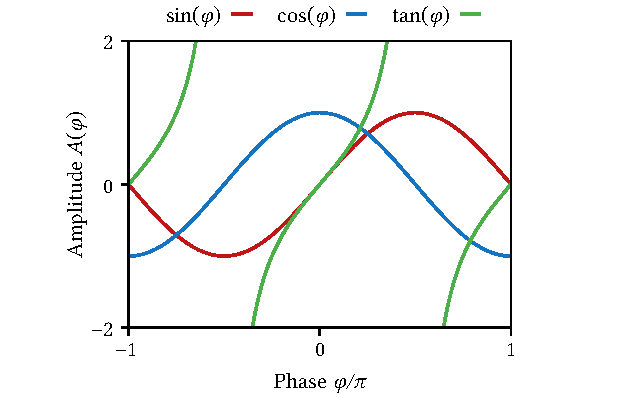
\includegraphics[width=0.2\textwidth]{test.jpg}
  \caption{This is simply a test figure, and some equation $\sin(2x)=1$, and some SI unit \SI{1.0e3}{m/s}, and some chemical \ce{CrO2}. This text can even be made even longer, since we want to test this properly.}
  \label{fig:test}
\end{figure}


Morbi non tortor volutpat, mattis odio at, tincidunt libero.
Donec pulvinar et mi at varius.
Sed vulputate lectus eu libero gravida, vel porta tortor bibendum.
Quisque dictum ex id quam ultrices, ut commodo nisl euismod.
Aliquam vulputate, urna quis sodales rhoncus, orci metus pulvinar velit, feugiat sollicitudin dui massa interdum tortor.
Nam sed ante vitae eros imperdiet bibendum.
Fusce pretium semper leo eget lobortis.
Sed dictum erat quis diam faucibus bibendum.
Integer vitae enim euismod, ornare augue quis, pharetra ante.
Phasellus venenatis tellus ut velit faucibus, posuere porttitor lacus hendrerit.

\begin{table}[h!]
  \centering
  \caption{This is simply a test table.}
  \label{tab:test}
  \begin{tabular*}{\dimexpr\textwidth-4em\relax}{@{\extracolsep{\stretch{1}}\,}lcc@{\,}}
    \toprule
    Name    &   Symbol    &   Value             \\
    \midrule
    Euler constant          & $e$   & $2.71...$  \\
    Circle constant         & $\pi$ & $3.14...$ \\
    Imaginary identity      & $i$ & $\sqrt{-1}$ \\
    \bottomrule
  \end{tabular*}
\end{table}

Lorem ipsum dolor sit amet, consectetur adipiscing elit.
Donec malesuada magna sem.
Fusce vitae lectus id magna convallis euismod.
Quisque viverra sollicitudin turpis, vel ultricies mauris dictum quis.
Praesent justo nunc, luctus in lectus in, placerat tempus orci.
Donec placerat neque ac tortor dignissim pellentesque.
Aenean tellus erat, eleifend id interdum a, volutpat et massa.
Quisque tristique accumsan efficitur.

Morbi non tortor volutpat, mattis odio at, tincidunt libero.
Donec pulvinar et mi at varius.
Sed vulputate lectus eu libero gravida, vel porta tortor bibendum.
Quisque dictum ex id quam ultrices, ut commodo nisl euismod.
Aliquam vulputate, urna quis sodales rhoncus, orci metus pulvinar velit, feugiat sollicitudin dui massa interdum tortor.
Nam sed ante vitae eros imperdiet bibendum.
Fusce pretium semper leo eget lobortis.
Sed dictum erat quis diam faucibus bibendum.
Integer vitae enim euismod, ornare augue quis, pharetra ante.
Phasellus venenatis tellus ut velit faucibus, posuere porttitor lacus hendrerit.

Lorem ipsum dolor sit amet, consectetur adipiscing elit.
Donec malesuada magna sem.
Fusce vitae lectus id magna convallis euismod.
Quisque viverra sollicitudin turpis, vel ultricies mauris dictum quis.
Praesent justo nunc, luctus in lectus in, placerat tempus orci.
Donec placerat neque ac tortor dignissim pellentesque.
Aenean tellus erat, eleifend id interdum a, volutpat et massa.
Quisque tristique accumsan efficitur.


\section{Continuation}
Morbi non tortor volutpat, mattis odio at, tincidunt libero.
Donec pulvinar et mi at varius.
Sed vulputate lectus eu libero gravida, vel porta tortor bibendum.
Quisque dictum ex id quam ultrices, ut commodo nisl euismod.
Aliquam vulputate, urna quis sodales rhoncus, orci metus pulvinar velit, feugiat sollicitudin dui massa interdum tortor.
Nam sed ante vitae eros imperdiet bibendum.
Fusce pretium semper leo eget lobortis.
Sed dictum erat quis diam faucibus bibendum.
Integer vitae enim euismod, ornare augue quis, pharetra ante.
Phasellus venenatis tellus ut velit faucibus, posuere porttitor lacus hendrerit.

Lorem ipsum dolor sit amet, consectetur adipiscing elit.\cite{feynman,statistics}\footnote{test}
Donec malesuada magna sem.
Fusce vitae lectus id magna convallis euismod.
Quisque viverra sollicitudin turpis, vel ultricies mauris dictum quis.
Praesent justo nunc, luctus in lectus in, placerat tempus orci.
Donec placerat neque ac tortor dignissim pellentesque.
Aenean tellus erat, eleifend id interdum a, volutpat et massa.
Quisque tristique accumsan efficitur.

Morbi non tortor volutpat, mattis odio at, tincidunt libero.
Donec pulvinar et mi at varius.
Sed vulputate lectus eu libero gravida, vel porta tortor bibendum.
Quisque dictum ex id quam ultrices, ut commodo nisl euismod.
Aliquam vulputate, urna quis sodales rhoncus, orci metus pulvinar velit, feugiat sollicitudin dui massa interdum tortor.\footnote{This is another footnote test.} %\footnote{This is simply just a simple test, with an equation $\sin \alpha = \cos(2a-1)/\cos(2a+1)$. And here is a chemical element \ce{CrO23} and physical unit \SI{12e3}{m}. }\footnote{Here is another footnote, also set in sans-serif.}%\footnote{$ABCDEFGHIJKLMOPQRSTUVWXYZ$ $abcdefghijklmopqrstuvwxyz$ $\alpha\beta\gamma\delta$ $\Gamma\Delta$ $\int_0^\infty \mathrm{d}x\,\sum_{ij} f(x_{ij}) \leq 0 \mathbf{xyz} \hat{x}+\check{y}\cdot\bar{u} \mathcal{F} \mathbf{x\sigma}$ $\sin x$  $\cos x$}
Nam sed ante vitae eros imperdiet bibendum. 
Fusce pretium semper leo eget lobortis.
Sed dictum erat quis diam faucibus bibendum.
Integer vitae enim euismod, ornare augue quis, pharetra ante.
Phasellus venenatis tellus ut velit faucibus, posuere porttitor lacus hendrerit.

Lorem ipsum dolor sit amet, consectetur adipiscing elit.
Donec malesuada magna sem.
Fusce vitae lectus id magna convallis euismod.
Quisque viverra sollicitudin turpis, vel ultricies mauris dictum quis.
Praesent justo nunc, luctus in lectus in, placerat tempus orci.
Donec placerat neque ac tortor dignissim pellentesque.
Aenean tellus erat, eleifend id interdum a, volutpat et massa.
Quisque tristique accumsan efficitur.

Morbi non tortor volutpat, mattis odio at, tincidunt libero.
Donec pulvinar et mi at varius.
Sed vulputate lectus eu libero gravida, vel porta tortor bibendum.
Quisque dictum ex id quam ultrices, ut commodo nisl euismod.
Aliquam vulputate, urna quis sodales rhoncus, orci metus pulvinar velit, feugiat sollicitudin dui massa interdum tortor.
Nam sed ante vitae eros imperdiet bibendum.
Fusce pretium semper leo eget lobortis.
Sed dictum erat quis diam faucibus bibendum.\footnote{Test}\cite{particle}
Integer vitae enim euismod, ornare augue quis, pharetra ante.
Phasellus venenatis tellus ut velit faucibus, posuere porttitor lacus hendrerit.
